\begin{minipage}{.5\linewidth}
	\begin{flushleft}
		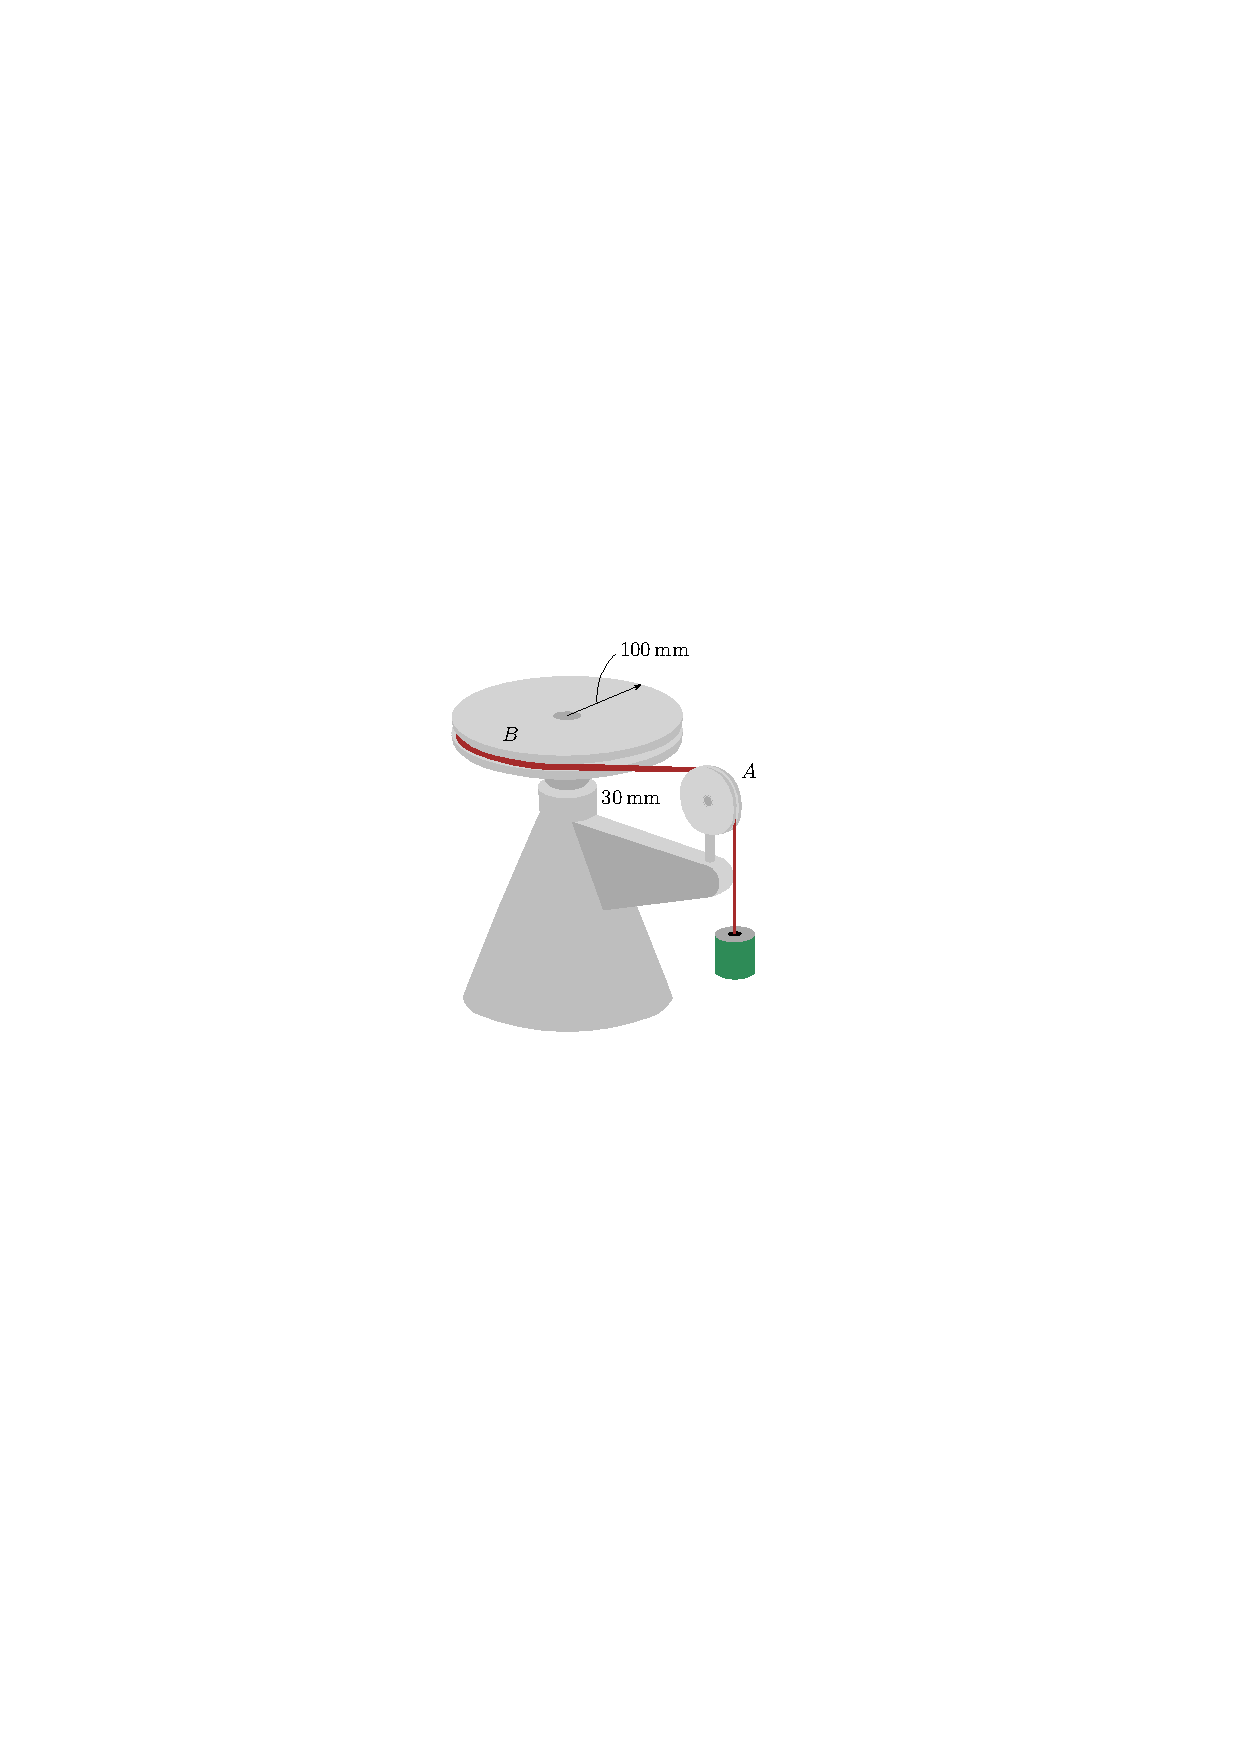
\includegraphics[scale=1.2]{../../images/draw_6_1}
	\end{flushleft}
\end{minipage}
\begin{minipage}{.5\linewidth}
	\vspace{-1cm}
	\item A montagem consiste de uma polia $A$, de \SI{3}{\kilogram}, e uma polia $B$, de \SI{10}{\kilogram}. Se um bloco de \SI{2}{\kilogram} está suspenso pela corda, determine a velocidade do bloco após ele haver descido \SI{.5}{\meter}, partindo do repouso. Despreze a massa da corda e trate as polias como discos finos. Não ocorre deslizamento.
\end{minipage}